\documentclass[12pt]{jarticle}
\usepackage[dvipdfmx]{graphicx}

% 文献番号や目次がハイパーリンク化
\usepackage[dvipdfmx]{hyperref}

% 表の幅指定
\usepackage{multirow}

% 余白の設定
\usepackage[top=30truemm,bottom=30truemm,left=25truemm,right=25truemm]{geometry}

%外字表示よう
%\usepackage{utf}

\makeatletter
\def\thefigure{\thesection.\arabic{figure}}
\@addtoreset{figure}{section}

\renewcommand\section{\@startsection {section}{1}%section周りのスペース
{\z@}%
{1.5\Cvs \@plus.5\Cdp \@minus.2\Cdp}%
{.5\Cvs \@plus.3\Cdp}%
{\reset@font\LARGE\bfseries}}%文字サイズフォント

\renewcommand\subsection{\@startsection {subsection}{2}%subsection周りのスペース
{\z@}%
{1.5\Cvs \@plus.5\Cdp \@minus.2\Cdp}%
{.5\Cvs \@plus.3\Cdp}%
{\reset@font\Large\bfseries}}%文字サイズフォント

\renewcommand\subsubsection{\@startsection {subsubsection}{3}%subsubsection周りのスペース
{\z@}%
{1.5\Cvs \@plus.5\Cdp \@minus.2\Cdp}%
{.5\Cvs \@plus.3\Cdp}%
{\reset@font\large\bfseries}}%文字サイズフォント
\makeatother


\begin{document}

% 著者,タイトル等
\begin{table}[h]
	\begin{center}
	{\renewcommand\arraystretch{1.3}
			\begin{tabular}{|c|c|c|c|c|c|} \hline
				題目 & \multicolumn{5}{c|}{移動を伴う現実環境でのテレイグジスタンス手法の提案と実装}\\
				\hline
			    学籍番号 & T31703M & 氏名 & 畑中衛  &  指導教員 & 濱川礼 \\
				  \hline
			\end{tabular}
	}
	\end{center}
\end{table}


% 概要(アブストラクト)
\input{sections/002_abstract}
\clearpage

\label{sec:start}

% 目次
%1
% 目次の表示
\tableofcontents

\clearpage

%1 担当
%%1
\section{担当範囲}

各員の担当を, 表\ref{担当範囲表} に示す.  
また, 各範囲の詳細は以下の章に記す. 

\begin{table*}[h]
	\centering
 	\begin{tabular}{|c|c|c|} \hline
		担当範囲 & 担当者 & 担当詳細 \\ \hline
		生活リズム推定部 & 畑中衛 & \ref{sec:rhythm} \\ \hline
		時刻変化設定部 & 菊地慎之介 & \ref{sec:setting} \\ \hline
		表示デバイス部 & 野地遼一 & \ref{sec:display} \\ \hline
 	\end{tabular}
	\caption{担当範囲表}
	\label{担当範囲表}
\end{table*}

%\clearpage

%2 概要
%2 概要
\section{概要}
本論文では現実空間を移動しながら遠くにいる友人と共に遠隔地の風景での行動を可能にするテレイグジスタンス 手法を提案し,その手法を基に実装した遠隔旅行システムについて述べる.

自身を遠隔地に存在しているかのようにするテレイグジスタンスという技術が存在する. この技術を利用し工場での作業やスポーツ観戦,旅行などを遠隔地から行う研究が行われている. これらの研究の多くは人型のロボットや完全没入型 VR を利用しており, 高い没入感での体験が可能であるが, ユーザの周囲の状況が判断できないために自由な移動ができない. 

これらの問題を解決するために透過型 MR ヘッドマウントディスプレイを用いてユーザをアバターとして遠くにいる友人の周りに表示し,さらに遠隔地の風景と現実の風景を重畳し,遠隔地の道路部分と現実の道路以外の部分を切り抜く手法を提案する. 

提案手法を基に遠隔旅行をするシステムを実装した.
システムにより複数のユーザ達は自分以外のアバターと共にあたかも遠隔地での旅行体験が可能となる. ユーザのアバターはヘッドマウントディスプレイの位置と同期しており, ユーザが移動を行うとアバターも同様に移動を行う. 遠隔地の風景表示は全天球パノラマ画像を用いてユーザ周囲の風景に重畳する. その際に視野確保のため道路部分を切り取る. これにより現実の道路を視認可能になり他者との衝突などの危険を抑制し現実空間での移動を可能にする.

本システムを評価するため学生10名に対し実験を行なった.
実験は本システムと関連したシステムのHoloTourを被験者に使用してもらい,その後テレイグジスタンスシステムの有用性の評価に使用される Presence Questionnaire と個人の没入感の感じ方を調べるのに使用される Immersive Tendencies Questionnaire という2つのアンケートに回答してもらった.
結果,本システムと HoloTour に有意差は見られなかったが,没入感を感じにくいほど本システムを使用した時遠隔地をよりリアルに感じることがわかった. 
\clearpage

%3 背景・目的
%3 背景・目的
\section{はじめに}
\subsection{背景}
遠隔地に自身が存在するかのような体験を可能にする, テレイグジスタンスという技術が存在する\cite{telexistence}.
この技術を利用し工場での作業やスポーツ観戦,旅行などを遠隔地から行う研究が行われてきた\cite{factorio}\cite{sprots}\cite{oculus}.

これらの研究の多くは図\ref{figure:Holopotation}のようなユーザの3Dモデル,または図\ref{figure:vrmodel}のようなロボッや完全没入型VRを利用することで自身の存在を遠隔地に投影させたり高い没入感で遠隔地で行動しているかのような体験を可能にしている\cite{vrmodel}\cite{ogasawara}.しかしこれらの手法においてユーザは移動しながら遠隔地での体験をすることはできない.ユーザの3Dモデルを利用する方法ではユーザ自身が深度情報を取得できるカメラに写っている必要があるためユーザの移動範囲に制限がある.
さらにロボットを用いた手法はユーザが完全没入型VRを利用する必要があり,ユーザは周囲の状況を把握することができないため移動しながらの利用はできない.

我々はこれらの問題を解決し実際に移動しながら遠隔地での体験を行うことでよりリアルな体験が可能になると考えた.
本研究では遠くにいる人と共に遠隔地の風景での行動を可能にする手法を提案する.そして提案した手法を基に遠くにいるユーザと共に遠隔旅行をするシステムの構築を行う.
本手法ではバーチャルヒューマンと呼ばれる仮想的な人間の3Dモデルをユーザのアバターとして使用することで自身の3Dモデル生成のための移動制限を無くす.更に出力に透過型MRヘッドマウントディスプレイを用いることで周囲の環境を認識し衝突などの危険性を抑制し,移動しならがリアルな体験を可能にする.

\begin{figure}[htbp]
\begin{center}
\includegraphics[width=16cm]{img/01_background/usermodel.eps} 
\end{center}
\caption{ユーザの3Dモデルを利用した手法}
\label{figure:Holopotation}
\end{figure} 

\begin{figure}[htbp]
\begin{center}
\includegraphics[width=16cm]{img/01_background/robovr.eps} 
\end{center}
\caption{ロボットや完全没入型VRを利用した手法}
\label{figure:vrmodel}
\end{figure} 

\clearpage

\subsection{目的}
本研究では移動を伴う環境において,テレイグジスタンスにより遠くにいる友人と,あたかも遠隔地で行動しているかのような体験をすることができる手法を提案し,提案手法を基に遠くにいるユーザと遠隔旅行をするシステムの開発を目的とする.

%睡眠不足は現代社会における深刻な問題である.

%睡眠不足によって記憶障害の原因となるたんぱく質が蓄積されることから, 睡眠不足はアルツハイマーの原因であると考えられている\cite{alzheimer}.
%さらに,睡眠時間が6時間以下の人は7時間の人に比べ死亡率が2.4倍になるという研究も存在する\cite{deadchance}.
%平成27年に厚生労働省が発表した調査では現代の日本人の40\%近くが睡眠時間6時間未満である.
%これは平成17年の調査結果より6\%増加しており, 日本人の睡眠時間は減少傾向にある\cite{undersix}.

%この問題の解決について, これまで様々なアプローチがとられてきた. だが, それらの多くは, 睡眠の「質」を向上させることを目的としている.
%代表的なものとして, レム睡眠, ノンレム睡眠のサイクルから最適なタイミングで起床を促す快眠支援アプリ「Runtastic Sleep Better」や, ユーザ固有の睡眠リズムから最適な音楽を流し睡眠の質を高める枕型デバイス「クローナ」などがある.

%我々は, この睡眠不足問題の改善のためには, 睡眠の「質」のみならず, 「量」をも重要視したアプローチをとることが重要であると考えた.

%なぜなら, ベネッセ教育総合研究所が行った調査「調査データクリップ!子どもと教育」において寝不足の理由の 50 \%以上が「なんとなく夜更かししてしまう」という結果が出たためである\cite{nebusoku}.
%「なんとなく夜更かししてしまう」のを改善するためには, ユーザに「寝なければいけない」という意識を持たせるよう働きかけること, 及び早めに就寝できるよう生活リズムを改善していくことが重要である.
%また, 「潜在的睡眠不足」と呼ばれる無自覚な睡眠不足に陥っている現代人が増加傾向にあることが, 国立精神・神経医療研究センターの調査により明らかとなっている\cite{psd}.
%潜在的睡眠不足に陥ると, 睡眠不足を自覚できないまま短時間の睡眠を繰り返し, 心身に負担を生じさせ続けてしまう. これの解消には, 睡眠の質を高めるアプローチよりも, 単純に長時間の睡眠を確保することが重要である.

%十分な睡眠時間を確保させるにはどうしたらよいか, という問題に対し, 我々は人々に時間を錯覚させることにより, 就寝時間を自然に早めさせることが可能なのではないか, という着想を得た.
%そこで我々は, 時間の錯覚効果が就寝時刻を早めるのに有効かどうか独自で調査を行った.

%調査協力者には, ゼミ活動での進捗報告会において時計を隠した状態で30分間過ごした後, アンケートで経過時間を回答してもらった. 男女 23 人を対象に調査を行った結果, 調査対象者の時間感覚に大きなばらつきが生じた.
%また, 日を改め, 時計を隠した状態で現在時刻を問い, そう思った理由を回答してもらったところ, 「ゼミ活動の進行度から類推した」「途中入室者の入室時間から類推した」など, 外的要因から時刻を類推した回答者が多く見受けられた.

%この2つの調査結果から, 人の時間感覚には個人差があり, 普段は日の高さや時計など外的要因により時間を知覚していると考えられる.
%この仮定は, 既存の研究\cite{study4}やフィクションのトリックなどにも用いられる\cite{clocktower}程, 普遍的な知見である.

%我々は以上の理由から, 外的要因を操作することでユーザに時間の錯覚を誘発させ, 就寝時刻を早めるシステムを開発した.
%なお, このシステムは就寝前の日が落ちた後に使用するシステムであるため, 外的要因として日の高さではなく, 時計表示に焦点をあて開発を行った.

\clearpage

%4 提案手法
%5 提案手法
\section{提案手法}
本研究の目的は移動を伴う環境において,テレイグジスタンスにより遠くにいる友人と,あたかも遠隔地で行動しているかのような体験を可能とする手法を提案し,提案手法を基に移動しながら遠くにいる友人と遠隔旅行をするシステムを開発することである.目的実現のために他ユーザの表示と遠隔地の風景表示を行う.
しかし移動しながらシステムを使用する場合に達成すべき課題が2つある.
1つはシステムを使用する際に周囲の環境を認識できることである.
本手法では遠隔地の風景を表示する際に道路部分は現実の風景を表示し,道路以外の部分のみ遠隔地の風景を表示することでユーザが周囲の状況を把握しながら遠隔存在することを可能にする.
2つ目はユーザがどれだけ移動しても遠隔地でユーザの存在が投影され続けることである.そのため本手法では自身の存在を遠隔地に投影させるために自分の3Dモデルではなくアバターを遠隔地に投影することでカメラの撮影範囲などの移動制限を無くし現実環境を際限なく移動可能にする.
これらの手法を実装したシステムによって遠くにいるユーザと遠隔旅行をする際,実際に移動しながらの体験が可能となる.

%我々はこれらの手法の有効性を評価するため,遠隔地の風景での行動を遠くにいる友人と共に体験することを可能にするシステムを開発した.
%開発したシステムはMRを用いて他ユーザをアバターとして表示し,遠隔地風景のパノラマ画像を表示する.
%これにより遠隔地の風景を見ながら表示された他ユーザのアバターと共に行動ができる.
\clearpage

\subsection{他ユーザの表示}
遠くにいる他ユーザを表示することで,1人で行動する際にあたかも複数人で一緒に行動しているかのような体験を可能にする.

%遠くにいる友人と行動しているかのような体験をするために,離れた場所にいる他ユーザのアバターを表示する.
\subsubsection{アバターの表示}
遠くにいる他ユーザを表示する際自身の3Dモデルなどではなくバーチャルヒューマンをユーザのアバターとして表示することで,自分自身の3Dモデル生成するためにカメラやKinect\cite{kinect}に写る必要がなくなる.その結果制限無く自由に移動することが可能となる.%本手法で扱うアバターはバーチャルヒューマンと呼ばれその存在が人の認知に対し影響を与えることがわかっている\cite{virtualhuman}.

\subsubsection{表示する他ユーザの選択}
表示する他ユーザは自分と同じ場所を遠隔地として指定したかによって選択する.
図\ref{figure:avatershare}は2人のユーザが同じ場所を遠隔地として指定した時の例である.
名古屋にいるユーザ1が遠隔地として指定したローマのコロッセオを,ロサンゼルスにいるユーザ2も同様に遠隔地として指定しているため,ユーザ1の視点には遠くにいるユーザ2のアバターが見える.逆も同様である.これにより他ユーザと一緒に行動することが可能となる.
%ユーザ同士のマッチングをユーザが指定した遠隔地の座標を比較し,距離が近いユーザがいた場合に行う.そしてマッチングされたユーザのアバターを表示する.
この時のユーザ同士を引き合わせる処理はオンラインゲームでRoomと呼ばれるサーバにユーザを接続し同期処理を行うPhoton Unity Cloud を利用した\cite{photon}.
これによりユーザはあたかも複数人でいるかのように感じることが可能となる.

\begin{figure}[htbp]
\begin{center}
\includegraphics[width=11cm]{img/02_proposedmethod/shareava.eps} 
\end{center}
\caption{他ユーザのアバター表示}
\label{figure:avatershare}
\end{figure} 

\clearpage

\subsubsection{アバターの動き}
アバターとユーザの位置と向きを同期することで,ユーザが移動した際にアバターも同様に移動する.ユーザとアバターの同期はヘッドマウントディスプレイの自己位置推定機能を用いて取得した端末の座標と方向を用いて行う.
この時アバターの方向は水平方向の変化のみ同期する.これによりユーザが上を見上げた時アバターが倒れることを防ぐ.

\clearpage





%\begin{figure*}[t]
%\begin{center}
%\includegraphics[width=17cm]{img/useimage.eps} 
%\end{center}
%\caption{風景重畳:(a)遠隔地の設定画面.(b)システムを使用イメージ.(c)出力イメージ}
%\label{figure:useimage}
%\end{figure*} 

\subsection{風景重畳}
%またユーザが風景を見る時は実際に歩くため,身体的動作の不一致によるVR酔いを抑制できる.
遠隔地で行動しているかのような体験をするために遠隔地の風景を360度パノラマ画像として取得し道路部分を切り抜き現実の風景に重畳表示する.これによりユーザの周囲の風景の道路以外の部分を変化させる.図\ref{figure:changescenery}に本手法を用いて豊田市の風景に対し,ローマのコロッセオの風景を重畳した例を示す.現実地風景(豊田市)は道路以外の部分が切り抜かれ,遠隔地風景(ローマのコロッセオ)は道路部分が切り取られている.切り取りを行なった2つの風景を重畳することで道路部分は現実地風景(豊田市),道路以外の部分は遠隔地風景(ローマのコロッセオ)が表示される.

\begin{figure}[htbp]
\begin{center}
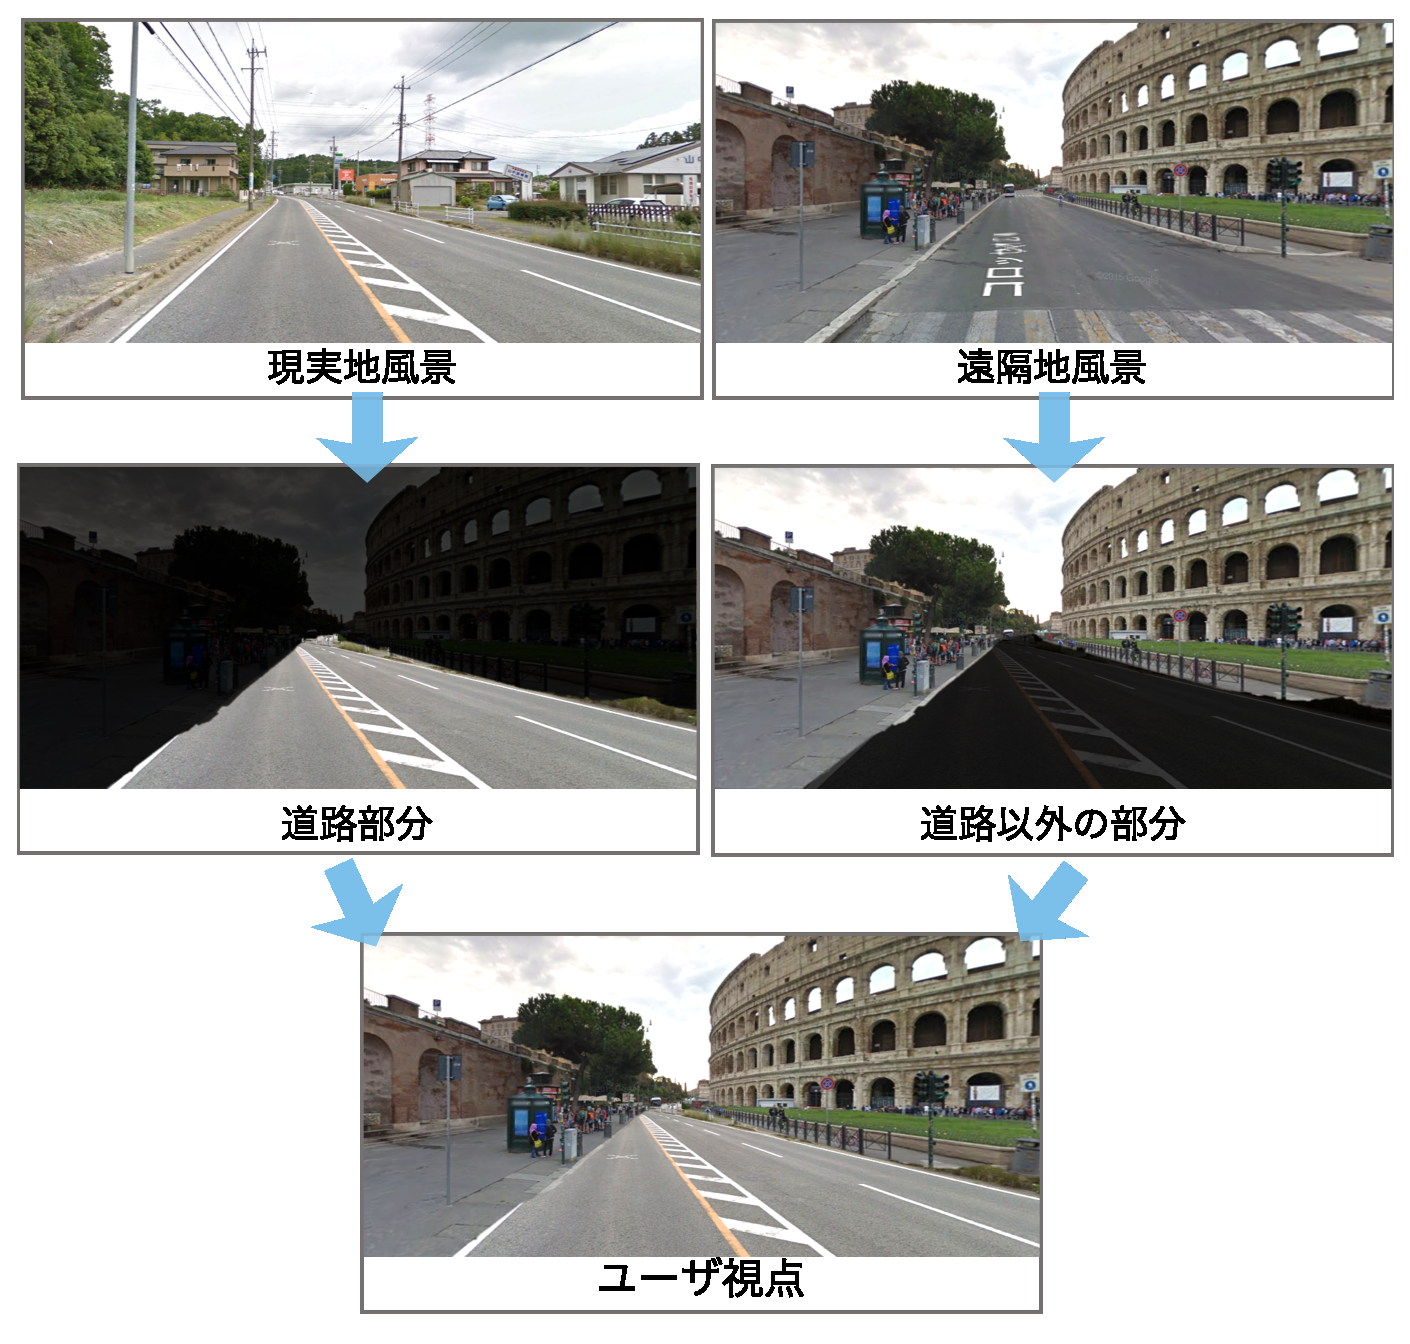
\includegraphics[width=11cm]{img/02_proposedmethod/changescenery.eps} 
\end{center}
\caption{風景変化}
\label{figure:changescenery}
\end{figure} 

\clearpage


\subsubsection{風景表示}
遠隔地の360度パノラマ画像を用いてユーザ周囲の風景を変化させる.パノラマ画像は GoogleStreetView\cite{gsv} を複数の視線の向きで取得した画像を結合することで取得する.
取得したパノラマ画像を球体型のオブジェクトの表面にテクスチャとして貼り付け,球体オブジェクトの内側に視点を置く事で周囲の風景を変化させる.ローマのコロッセオのパノラマ画像を生成し,球体オブジェクトに貼り付け内側から見た様子を図\ref{figure:sphere}に示す.

\begin{figure}[htbp]
\begin{center}
\includegraphics[width=16cm]{img/02_proposedmethod/scenery_change.eps} 
\end{center}
\caption{パノラマ画像の取得と表示手法}
\label{figure:sphere}
\end{figure} 

\clearpage

\subsubsection{道路部分の切り抜き}
球体オブジェクトにパノラマ画像を貼り付けるだけではユーザの視線を覆ってしまうため,歩行者や自転車などと衝突する危険性がある.そこで本手法では図\ref{figure:trimroad}のように重畳表示する風景の道路部分を切り抜くことで道路部分のみ現実の道となり衝突の危険を抑制する.
道路部分の切り抜きにはマスク処理を用いる.
マスク画像は事前に手動で風景のパノラマ画像の道路部分を黒くし, 風景部分を白くすることで作成する.

\begin{figure}[htbp]
\begin{center}
\includegraphics[width=16cm]{img/02_proposedmethod/overlay.eps}
\end{center}
\caption{風景重畳:(a)現実の風景.(b)ユーザが指定した遠隔地の風景.(c)遠隔地の風景から道路部分切り抜き.(d)重畳.}
\label{figure:trimroad}
\end{figure} 

\clearpage


\subsubsection{遠隔地と現実の歩行コースマッピング}
現実で歩くコースと指定した遠隔地のコースは曲がり角やカーブなどの構造が異なる.そこで本手法はユーザの進行方向を元に遠隔地の風景の向きを操作することで,常にユーザが移動する方向へと道路が続くように風景の表示を行う.更新前と更新時のユーザの座標を元にユーザの進行方向を算出し,それを元に風景表示用の球体オブジェクトの向きを調整する.ユーザの進行方向と風景の向きの調整を図\ref{figure:landscape_rotate}に示す.図\ref{figure:landscape_rotate}(a)のように画像奥方向に進んでいる時,遠隔地風景から切り取った道路部分はユーザの進行方向と同様に画像奥方向へ続く.その後ユーザが進行方向を変え,図\ref{figure:landscape_rotate}(b)のように右方向に進行するとそれに合わせ遠隔地の道路部分も右方向へ続く.これにより常にユーザの進行方向へと道が続き,ユーザが歩いている道が遠隔地の風景の切り抜き部分に表示される.

\begin{figure}[htbp]
\begin{center}
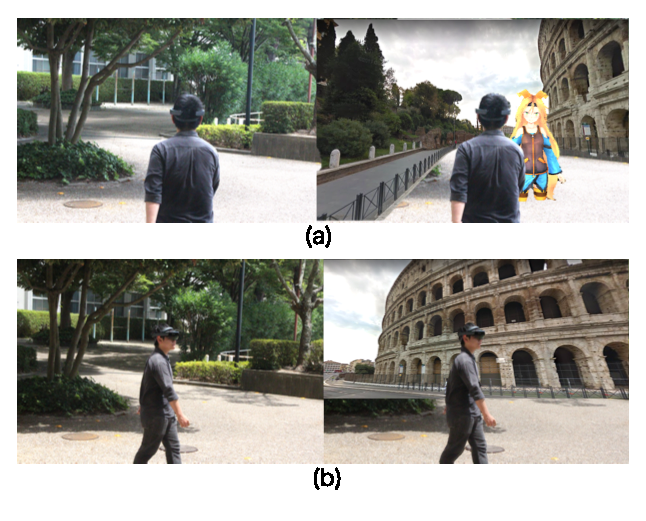
\includegraphics[width=11cm]{img/02_proposedmethod/user_dire.eps} 
\end{center}
\caption{(a)奥に向かい歩くと道が奥に続く.(b)歩く方向を変えると道が続く方向も変わる}
\label{figure:landscape_rotate}
\end{figure} 

%この時道路部分のみ現実の風景を表示することで,他の歩行者や乗用車などと衝突する危険を抑制する.
%重畳イメージを図\ref{figure:changescenery}に示す.
%図\ref{figure:changescenery}においてシステムを通してユーザがみている風景の道路部分は現実地風景の道路部分が表示されており,道路以外の部分は遠隔地の風景が表示されている.これによりユーザは現実の道路を視認しながら遠隔地の風景を楽しむことができる.
%本手法を実装するため遠隔地の風景を360度パノラマ画像として取得し,球体オブジェクトに貼り付けることでユーザの周囲の風景を変化させる.図\ref{figure:sphere}にローマのコロッセオの風景をパノラマ画像として取得し,球体オブジェクトを貼り付けた例を示す.














%従来睡眠を支援するアプリケーションは, 前述したとおり睡眠の質を向上させるものが多かった. 

%しかし, 2016年の研究で, 現代人の多くが自覚できない睡眠不足(潜在的睡眠不足)を抱えていることが明らかになった\cite{psd}.
%この原因として, 被験者の習慣的睡眠時間が必要睡眠量よりも平均1時間ほど短いことがあげられた.
%この問題の改善には, 睡眠の質のみならず量をも充足することが必要である.

%そこで我々は時計の時刻を操作し, ユーザが知覚する時刻を早めることで, 睡眠量を確保できるシステムを開発した.

%\subsection{IllusionClock}
%IllusionClock では, 表示デバイス及び管理アプリケーションの画面に表示する時刻(以下, 表示時刻)を, 実際の時刻よりも早めることにより, ユーザに表示時刻が正しいものだと錯覚させる.

%ここで, 現実ではユーザが理想とする就寝時刻である瞬間に, IllusionClock ではユーザの普段の就寝時刻を表示することで, 普段通りの生活を送ろうと考えたユーザの理想の就寝時刻と実際の就寝時刻とを近づけることが出来る.


%\subsection{生活リズム推定}
%IllusionClock ではユーザの普段の就寝時刻を推定し, 記録している.
%ユーザは加速度センサを搭載している AndroidWear を手首に装着する(図\ref{fig:wearable}). アプリケーションを起動し(図\ref{fig:system}), 普段通りの生活を送るだけで, 普段の就寝時刻が記録される.




%\subsection{時間変化設定}
%IllusionClockでは, 時刻変化の設定をユーザが Android アプリケーションを介して行う(図\ref{fig:setting}). ユーザが設定できる項目は理想就寝時刻, 普段の就寝時刻, 変化曲線である. 普段の就寝時刻に関しては生活リズムの推定結果を反映させることが可能である.


\clearpage

%4 関連研究
\section{関連研究}
本研究を行うにあたり5つの点に着目し,関連する研究を紹介する. 1つ目は遠隔地にいる他ユーザを表示する点, 2つ目はバーチャルヒューマンを利用する点, 3つ目は風景を変化させる点, 4つ目は移動を伴う環境で使用する点, 5つ目はMRを利用している点である.以下紹介した研究と本研究との関係を述べる.

% + MR,移動を伴うシステム,バーチャルヒューマン

\subsection{他ユーザの表示をする研究}
ユーザの存在を遠隔地に表示させるためにユーザの3Dモデルを用いた手法が存在する.

濵上らは対話相手に自身の空間へと侵入されている感覚「被侵入感」を提示し,テレプレゼンスの向上を目指すビデオチャットシステム「ドアコム AR」を開発した\cite{doorcom}.
ドアコムARはKinectにより取得したユーザのカラー情報,深度情報から3次元点群データを取得する.
取得した点群データを遠隔地にいる別のユーザの前に表示することで同室感のあるビデオチャットが可能になる.
このようにユーザの姿を遠隔地に表示するシステムは他にも存在する.
CutlerらはHololens\cite{Hololens}を利用し遠隔地にいる友人の存在をリアルタイムで表示するシステムHolopotationを開発した\cite{holopotation}.
Holopotationは深度情報を取得可能なカメラを複数使いユーザを撮影し、ユーザの3Dモデルを作成する.
そして作成した3Dモデルを遠隔地にいる別のユーザの前にHololensを通して表示することで,遠隔地にいるユーザとコミュニケーションを取ることができる.

\clearpage

\subsection{バーチャルヒューマンを用いた研究}
本手法は他ユーザをアバターとして表示する.このようにコンピュータによって表示される人間はバーチャルヒューマンと呼ばれ,人の認知に与える影響が調査されている.

Devidらはユーザーの心理的苦痛に関連する情報を共有する,魅力的な対面式対話を作成するように設計された SimSensei Kiosk というバーチャルヒューマンのインタビュアーを開発した\cite{kiosk}.SimSensei Kioskはうつ病や不安といった心理的苦痛を自動評価することで,会話相手であるユーザに対し快適な会話や情報共有を可能とする.

デジタルエミリーというリアリティのあるバーチャルヒューマンが存在する\cite{digitalemily}.しかし人はこのようなリアリティのあるバーチャルヒューマンに対して不気味だと感じることがある.Maryamらはこうしたリアルなバーチャルヒューマンを見たときの人間の脳波を学習し,不気味と思うバーチャルヒューマンを調査した\cite{maryam}.

\clearpage

\subsection{風景を変化させる研究}
パノラマ画像を球体オブジェクトに貼り付け風景を変化させる手法はChenらによって提案され\cite{shenchang},その後この手法を用いたVR研究が多く行われるようになった.

RuygらはヘッドマントディスプレイOculus Riftを用いて Google Street View を表示する Oculus Google Street View を実装した\cite{oculus}.これによりユーザは Google Street View が存在する場所を表示し,あたかもその場所に行ったかのような体験が可能となる.

Calagariらはスポーツ放送のカメラ映像から広角パノラマ画像を生成することで没入型のスポーツ観戦システムを実装した.実装したシステムについて評価した結果ほとんどの評価参加者が没入感を感じた\cite{sprots}.

\clearpage

\subsection{移動を伴う環境で使用する研究}
移動を伴う環境で使用する研究として
Nguyen らはユーザがジョギングする際に過去の自分のスピードを元に生成された影を AR により走らせることで,ジョギングのモチベーション維持を図るシステム Fitnamo を提案している\cite{fitnamo}. このシステムは過去のユーザのジョギングデータを元に,ユーザ自身の平均速度, または最高速度で走る影をGoogleGlass に投影し,競争心を持たせることでモチベーションの動機付けを図っている. 
%図 3 はこの システムの使用例である. 赤く表示されているのは 今までのユーザの平均速度で走った場合のユーザの 位置を示している.

ナイアンティックと株式会社ポケモンはスマートフォン向け位置情報ゲームアプリケーションのポケモンGOを開発した\cite{pokego}.
ポケモンGOはスマートフォンのGPS機能を使用しながら移動することでキャラクターの捕獲・育成・交換・バトルを画面上で行うことができる。

\clearpage

\subsection{MRを用いた研究}
MRを用いた研究としてMichael らは複数人でチームを組み現実世界に投影した仮想ドローンを撃ち落とすMRマルチプレイヤーゲームを提案している\cite{mrgame}.Michaelらのシステムは屋外ゲームにおいて,プレイヤー間の相対的な位置を追跡することで複数人でのプレイを可能にした.相対的な位置の推定はGPSを用いて行っている. 

%差
本システムはパノラマ画像により周囲の風景全体を変化させることでよりMRとしての没入感の向上を図る.

HaleyらはHololensにより,ペルーのマチュピチュ遺跡やイタリアのナヴォーナ広場の環境音を流し,周囲の映像を表示することであたかもその場所に言ったかのような体験を可能にするHoloTourを開発した\cite{holotour}.環境音は指向性マイクを利用し録音し周囲の風景は$360^\circ$カメラを使い撮影した.

\clearpage

\subsection{関連研究との差異}
濵上ら,Cutlerらのシステムはリアルなユーザのモデルを表示可能であるが,自分がKinectやカメラに映る範囲にいなければならないため,移動範囲に制限が存在する.
本手法はユーザの存在をアバターとして表示し,その制御をHololensの自己位置推定機能により行なっているため,設置が必要な機器がなく移動範囲に制限を無くした.

DevidらやMaryamらはバーチャルヒューマンの研究を行なっている.本手法ではMRを用いてバーチャルヒューマンを表示することにより,ユーザが移動しながら自身の存在を遠隔地に表示する.

Ruygら,Calagariらのシステムは仮想空間の移動にコントローラを用いるか,移動せずその場で周りを見渡すことで仮想空間を体験する.これに対し本手法はMRを用いているためユーザは実際に歩きながら仮想空間の風景の中で行動ができる.これにより身体的動作を伴った体験になるためユーザはより現実感のある体験が可能になる.


NguyenらやMichaelら,ナイアンティックが開発したシステムはARやMRを用いて現実世界にオブジェクトを投影している.本手法では現実世界に対し遠隔地の風景を重畳することで,ユーザの周囲ほとんどが仮想の風景へと変化する.

Haleyらのシステムは高性能なカメラと指向性マイクにより没入感の高い体験が可能であるが,現実環境を視認できず移動範囲も制限がある.本システムは表示する遠隔地の風景から道路部分を切り抜くことで,現実の道路を視認可能にしている.そのため実際に移動しながら遠隔地に行ったかのような体験を可能にしている.

%\subsection{アウトドアレクリエーションの拡張}
%アウトドアレクリエーションを拡張するシステムとして屋外ゲーム,屋外ナビゲーションシステムについて述べる.
%屋外ナビゲーション
%Aysegul Dogangunらは身体活動を改善するための個別の推奨事項を生成するモバイルアプリケーションを開発した.[\cite{Aysegul}Aysegul Dogangun 2017]. このアプリケーションはユーザーが必要なすべての活動データを収集する.収集したデータに基づいて,アプリケーションは毎日のルーチンで不足した運動量を補完するために,毎日のルーチンよりも運動量が増加した活動を自動的に推奨する.
%Maaretostiらは,非自発的なハイキングシステムであるHOBBITを開発した[\cite{maaret} Maaret Posti 2014].このシステムはユーザが興味のある領域のハイキングコースを提案することに加え,ユーザ周辺のWi-Fi機器を検出し通知することで,ユーザが一人で歩くことを支援している.
%Aysegul DogangunらやMaaret Postiらはモバイル端末への活動量の通知や提案コースと周辺のユーザを通知する事でレクリエーションの拡張を図っている.
%本システムではMRを用いた視覚的情報の操作によるレクリエーションの拡張を図る.

%本システムと同様にMRを用いた手法としてMichael Bonfertらは複数人でチームを組み現実世界に投影した仮想ドローンを撃ち落とすMRマルチプレイヤーゲームを提案している[\cite{Michael}Michael Bonfert 2017].Michael Bonfertらのシステムは屋外ゲームにおいて,プレイヤー間の相対的な位置を追跡することで複数人でのプレイを可能にした.相対的な位置の推定はGPSを用いて行っている. 本システムはパノラマ画像により周囲の風景全体を変化させることでよりMRとしての没入感の向上を図る.
%位置付け
%屋外ゲーム
%Aysegulらは身体活動を改善するための個別の推奨事項を生成するモバイルアプリケーションを開発した\cite{Aysegul}. このアプリケーションはユーザーが必要なすべての活動データを収集する.収集したデータに基づいて,アプリケーションは毎日のルーチンで不足した運動量を補完するために,毎日のルーチンよりも運動量が増加した活動を自動的に推奨する.
%Maaretostiらは,非自発的なハイキングシステムであるHOBBITを開発した\cite{maaret}.このシステムはユーザが興味のある領域のハイキングコースを提案することに加え,ユーザ周辺のWi-Fi機器を検出し通知することで,ユーザが一人で歩くことを支援している.
%Aysegul DogangunらやMaaret Postiらはモバイル端末への活動量の通知や提案コースと周辺のユーザを通知する事でレクリエーションの拡張を図っている.
%本システムではMRを用いた視覚的情報の操作によるレクリエーションの拡張を図る.

%Devid Debultらはユーザーの心理的苦痛に関連する情報を共有する,魅力的な対面式対話を作成するように設計された Sim Sensei Kiosk というバーチャルヒューマンのインタビュアーを開発した.
%SimSensei Kioskはうつ病や不安といった心理的苦痛を自動評価することで,会話相手であるユーザに対し快適な会話や情報共有を可能とする.

%Maryam Mustafaらはバーチャルヒューマンが人の認知に与える影響を調査している.人はデジタルエミリーのようなリアリティのあるバーチャルヒューマンに対して不気味だと感じることがある.Maryam Mustafaらはこうしたリアルなバーチャルヒューマンを見たときの人間の脳波を学習し,不気味と思うバーチャルヒューマンを調査した.
%本システムでは,MRを用いてバーチャルヒューマンを表示することにより,ユーザがレクリエーションを行う際に複数人でのレクリエーション体験の演出を図る.

\clearpage

%5 事前検証
%\input{sections/045_pre-experiment}
%\clearpage

%5 システム構成
%5 システム構成
%\section{システム構成}
%IllusionClockは時計の時刻を操作し, ユーザに対して時間の錯覚を誘発させることで理想の就寝時刻を提供するシステムである.

%IllusionClockは, 生活リズム推定部, 時刻変化設定部, 表示デバイス部 の3つのモジュールによって構成されている. 図 \ref{system} に示す.
%このシステムでできることのみを書く
\section{遠隔旅行システム概要}

提案手法に基づき遠くにいるユーザと遠隔旅行を行うシステムを実装した.
実装にはゲーム開発エンジンUnityを使用し\cite{Unity},ヘッドマウントディスプレイはMicrosoft社のHololensを使用した\cite{Hololens}.
本システムの構成を図\ref{figure:system}に示す.
本システムはデータ取得部,風景生成部,出力部から構成されている.
データ取得部で取得したユーザIDと遠隔地情報は風景生成部に送られ,遠隔地情報を元にサーバ上にパノラマ画像を生成する.風景生成部で生成されたパノラマ画像は風景を更新する際に,ユーザIDを元に識別されたHololensの出力部へ送られる.出力部からは風景を更新するかを決定するためにユーザの位置情報を風景生成部に送っている.

\begin{figure}[ht]
 \begin{center}
  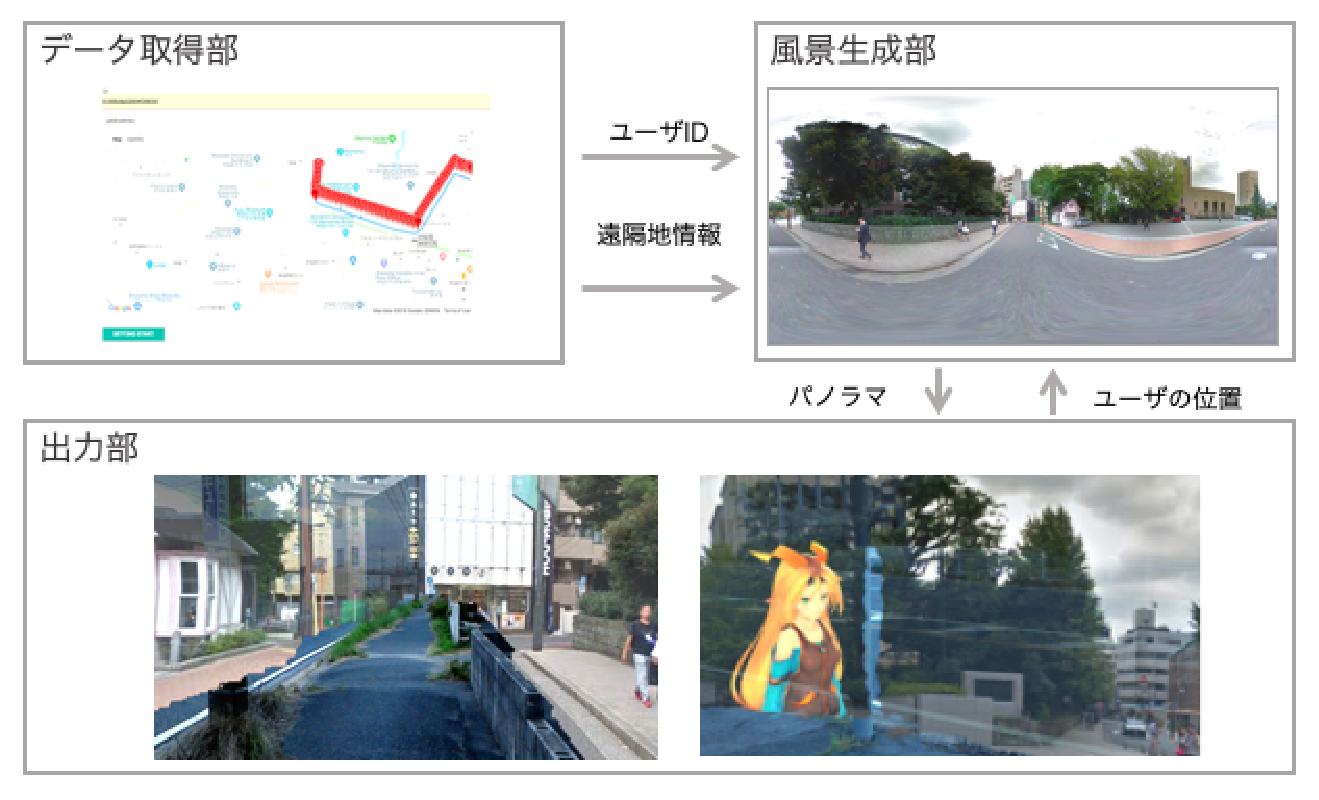
\includegraphics[width=16cm]{img/04_detail/system.eps}
  \caption{本システムの構成}
  \label{figure:system}
 \end{center}
\end{figure}

\clearpage
 
\subsection{システム利用イメージ}
本システムを利用する際,ユーザはまずHololensを装着し,風景表示を行うアプリケーションを起動する.起動した際に表示されるHololensの端末IDを,遠隔旅行を行うコース設定用Webページで入力する.その後Webページに表示されているマップ上をクリックする事で遠隔旅行コースの出発地点,目的地点を設定する.システムは出発地点と目的地点を繋ぐコースが生成し,コース上のパノラマ画像を取得する.パノラマ画像の取得が完了したら,Hololens上で遠隔地の風景が表示され遠隔旅行をする事が可能になる.
図\ref{figure:usecase}は遠隔地としてローマのコロッセオを設定し,遠隔旅行を体験している例である.

\begin{figure}[ht]
 \begin{center}
  \includegraphics[width=16cm]{img/04_detail/useimage.eps}
  \caption{システム利用イメージ}
  \label{figure:usecase}
 \end{center}
\end{figure}

\clearpage
% データ取得部
\subsection{データ取得部}
データ取得部は,出力部でのユーザ識別,ユーザ毎の風景表示のため,ユーザ情報,遠隔地のStreetViewに関する情報を取得する処理群である.データは遠隔地設定ページでユーザが入力した値を使用する.取得したデータはデータベースに保存し管理する.本システムではUnityの標準クラスで利用可能な軽量データ交換フォーマットJSONを利用しデータを管理する\cite{json}.
以下にJSONに含まれる各データの詳細を示す.

\begin{table}[ht]
  \begin{tabular}{| c | l |}
  \hline
    ユーザID & ユーザを識別するための固有ID \\ \hline
    表示遠隔地 & 遠隔地の情報からユーザが現在見ている遠隔地の場所を抽出するための値\\ \hline
    遠隔地の情報群 & 指定遠隔地の経度,緯度,パノラマID \\ \hline
  \end{tabular}
\end{table}

\clearpage

\subsubsection{ユーザ情報取得}
ユーザ情報取得部ではユーザの識別のために使用する固有のユーザIDを取得する.ユーザIDとしてユーザが使用するHololensの端末IDを使用する. 遠隔旅行をするコースの設定用Webページでユーザが入力したHololensの端末IDをサーバに送信し,データベースを更新する.これによりシステムを使用する際にどのユーザがどのアバターの制御するかを識別する.

\clearpage

\subsubsection{StreetView情報取得部}
コース設定部ではユーザが選択した 2つのポイ ントを出発地と目的地とし, 徒歩での移動コースを 生成する. コースの生成は GoogleMapsApi を用いて行なう\cite{googlemapsapi}. 
生成したコース上にStreetViewを取得する座標を一定の間隔で設定する.Google が定めた StreetView 認定要件において StreetView 間の距離は 3 メートルとなっていたため\cite{svrule}. コース上に設定するStreetViewを取得する座標の間隔は 3 メートルとした. StreetViewを取得する座標の設定方法はまずコース上からカーブや曲がり角を全て抽出し, それぞれの座標を記録する. その後抽出した座標間を 3 メートル間隔で分割し, StreetViewを取得する座標を設定する. 
その後Google Maps APIを用いて3メートル感覚で取得した座標からStreetViewのパノラマ画像が持つ固有のパノラマIDを取得する.取得したパノラマIDと座標をデータベースに書き込み更新をする.データベースへの書き込みは出発地点の座標からはじめ,同じパノラマIDを持つ座標は書き込みを行わないようにした.これによりデータベースでパノラマIDが重複する事を防ぐ.



%図\ref{figure:setcource}は

%図 9 の例ではコース上から 3 つの曲がり角の座標を記録し, 更に各座標間において 3 メートル間隔で StreetView を取得するポイントを計 78 ポイント設定している.



\clearpage

% 風景生成部
\subsection{風景生成部}
風景生成部はデータ取得部で取得したStreetViewの情報からパノラマ画像の生成,道路部分切り抜きを行い,出力部へと送る風景画像を生成する処理群である.
\subsubsection{パノラマ画像生成}
パノラマ画像の生成にはGSVPanoライブラリを利用した\cite{GSVpano}.GSVPanoライブラリはGoogleStreetView からパノラマ画像を作成するライブラリである.パノラマ画像の生成は図\ref{figure:panorama}のようにパノラマ表示されたGoogleStreetViewについて複数の視線の向きで28枚の画像を取得する.その後パノラマ画像になった時,隣接する部分の画像どうしを結合することで一枚のパノラマ画像を生成する.
その後システムは生成したパノラマ画像トリミングすることで余白部分の削除を行う.

\begin{figure*}[ht]
\begin{center}
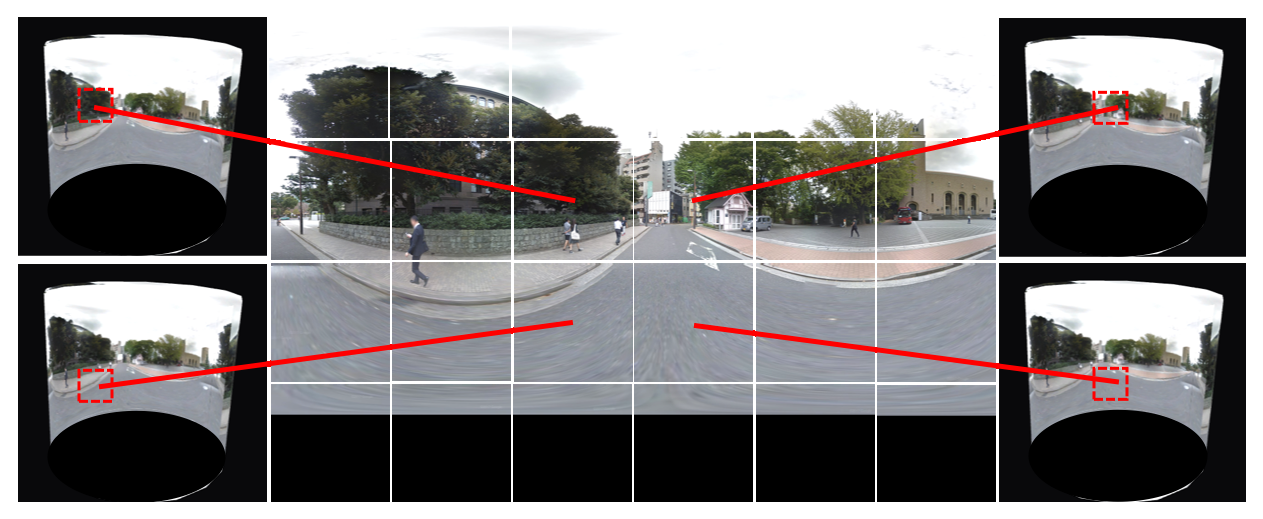
\includegraphics[width=17cm]{img/04_detail/make_panorama.eps}
\end{center}
\caption{パノラマ画像の生成}
\label{figure:panorama}
\end{figure*} 

\clearpage

\subsubsection{道路部分切り抜き}
StreetView 取得部で取得した画像に対し道路部の切り抜きを行う. 切り抜きにはマスク処理を用いる. マスク画像は事前に手動で StreetView の道路部分を黒くし, 風景部分を白くすることで作成した. StreetView取得部で取得した画像に対し図\ref{figure:trim}のようにマスク画像を用いてマスク処理を行い道路部分を切り抜く.


\begin{figure}[h]
\begin{center}
\includegraphics[width=11cm]{img/04_detail/triming.eps} 
\end{center}
\caption{マスク処理による道路部分の切り取り}
\label{figure:trim}
\end{figure} 
%\clearpage
\clearpage
% 出力部
\subsection{出力部}
出力部は風景生成部で生成したパノラマ画像とデータ取得部で取得したユーザ情報を元に風景,他ユーザの表示,またユーザの移動による風景の更新を行う処理群である. ユーザ A とユーザ Bがレクリエーションしている出力例を図\ref{figure:output}に示す.
(a),(b)はそれぞれ ユーザ A, ユーザ Bが実際にいる場所の風景である.(c) はユーザ A, ユーザ Bが遠隔旅行こーすとして設定した場所(東京)の風景を示している.(d)は ユーザ A, ユーザ Bが実際にいる場所と, 指定した遠隔地の位置関係である. (e)はユーザ Aから見える風景である.現実空間に遠隔地が重畳され,同じ遠隔地を指定したユーザ Bのアバターが表示されている.(f)は反対にユーザ Bから見える風景である. (g)はシステム使用時の遠隔地における二人のユーザの位置関係である.

\begin{figure*}[ht]
\begin{center}
\includegraphics[width=17cm]{img/04_detail/output.eps}
\end{center}
\caption{システム使用例と出力}
\label{figure:output}
\end{figure*} 

\subsubsection{風景表示}
現実風景への重畳は球体のオブジェクトにテクスチャとして風景生成部で生成したパノラマ画像を貼り付けることで行う.
パノラマ画像を貼り付けた球体オブジェクトの内部にシステム起動時ユーザの視点となるUnityのカメラオブジェクトを配置する.
これにより周囲の風景は遠隔地の風景へと変化する.


\clearpage

\subsubsection{他ユーザの表示}
他ユーザの表示ではユーザが表示している遠隔地が近い他ユーザのアバターを表示する.アバターとしてUnityのAsset Storeで無料配布されているUnityちゃんを使用した\cite{unitychan}.
ユーザ間のアバターの同期処理にはオンラインゲームの同期処理に使われる Photon Unity Cloud を利用した\cite{photon}.
表示するユーザはデータ取得部で生成したJSONデータを元に決定する.
システムはJSONデータのユーザ情報と現在地情報から,表示する遠隔地同士の距離が近いユーザのユーザIDを取得する.
そして取得したユーザIDを元にPhoton Unity Cloud のルームを検索する.ユーザは取得した近いユーザのIDと同じ名前のルームが存在する場合,入室する.検索した結果近いユーザのIDと同じ名前のルームがなければシステムは自身のユーザIDと同名のルームを作成する.
これにより他ユーザとのアバターの共有を行う.
アバターの向きはHololensの
$\it{y}$
軸方向のみ同期していおり,図 \ref{figure:abatar}(a)のようにアバターの回転を水平方向のみに制限している.またアバターの座標はHololensの座標と同期しており,図\ref{figure:abatar}(b)のようにユーザが進行した方向に動く.

\begin{figure}[h]
\begin{center}
\includegraphics[width=11cm]{img/04_detail/avatar_move.eps} 
\end{center}
\caption{アバターの動き}
\label{figure:abatar}
\end{figure} 

\clearpage

\subsubsection{風景更新}
風景更新ではユーザが歩くことでパノラマ画像を更新する.ユーザの位置はHololens の自己位置推定機能によって算出する.自己位置推定機能とはHololensのアプリケーション起動時の座標との相対距離を推定する機能である. HololensとUnityのカメラオブジェクトは座標と方向が同期されているため,カメラオブジェクトの座標を取得することで自己位置を推定が可能である.風景の更新はHololensが3メートル座標移動するごとに行う.これはGoogle が定めた StreetView 認定要件において StreetView 間の距離が3 メートルとなっていたためである.
システムは風景更新時のHololensの座標と,前回の更新時のHololensの座標から移動方向を算出し,ユーザの移動方向に道が続くように風景表示用の球体オブジェクトを回転させる.
移動方向の算出にはUnityのVector3クラスに定義されている,GetAim関数により算出できる.
%\clearpage

\clearpage

%6 評価・考察
%6 評価・考察
\section{評価・考察}
本章では, 実装した遠隔旅行システムと関連研究であげたHoloTourの比較,評価実験について述べる.

\subsection{評価手法}
実験は被験者10人に対して行なった.被験者は本システムと関連研究であげたHoloTourを使用して遠隔地の風景を体験した後アンケートに回答した.
この時システムを使用する順番はランダムに決定し,体験する遠隔地は2つシステムで同じ場所に統一する.
実験で体験する遠隔地はHoloTourで体験可能なイタリアのナヴァーナ広場とした.
本システムを使用する際被験者の前にアバターを表示し, 我々がノートパソコンを通してアバターを操作した.
%HoloTourで体験できる風景は現時点でペルーの世界遺産マチュピチュとイタリアのナヴァーナ広場のみであったため,同じ風景を
システム使用後に回答するアンケートはWitmerとSingerにより提案され,その後UQOサイバー心理学研究室により改訂されたPresence Questionnaire(PQ)と, Immersive Tendencies Questionnaire(ITQ)を利用し2つのシステムの比較を行う\cite{pq}\cite{itq}.
PQはプレゼンスシステムの優位性を測る質問であり,以下の項目を評価することでシステムの優位性を算出できる.

\begin{table}[ht]
 \begin{center}
  \begin{tabular}{| l |}
  \hline
 現実感高さ(現実感) \\ \hline
システムで行える行動のレベル(行動) \\ \hline
 表示や操作などの質(インタフェース) \\ \hline
 仮想環境でどれだけ探索や調査ができたか(調査)\\ \hline
 仮想環境での自身のパフォーマンスの熟練度(パフォーマンス)\\ \hline
 音響の質(音響)\\ \hline
 触覚フィードバックの質(触覚)\\ \hline
  \end{tabular}
  \end{center}
\end{table}
ITQは個人が感じる没入感の傾向を測る質問であり,スコアが高いほど没入感を感じやすいことを示している.
PQの結果について2標本$t$検定を行い比較を行うシステムの平均値に有意差が存在するか調査する.
この時有意水準を$0.05$とした.
またPQのスコアとITQのスコアの関係を調査し本システムの評価を行う.

比較は PQ から本システムに実装されていない音響と触覚に関する項目を抜いた現実感,行動,インタフェース,調査,自身のパフォーマンスの5項目について行う.
PQの質問は合計19問で,それぞれ7段階で評価してもらった.
スコアは原著論文の方法通り現実感,行動,調査,自身のパフォーマンスはスコアが高い方が優れている事とし,逆にインタフェースはスコアが低い方が優れている事とする.

\clearpage

\subsection{評価結果}

各項目について本システムとHoloTourを比較した結果を図\ref{figure:pqresult}に示す.図に関しての説明を以下に示す.

\begin{figure}[h]
\begin{center}
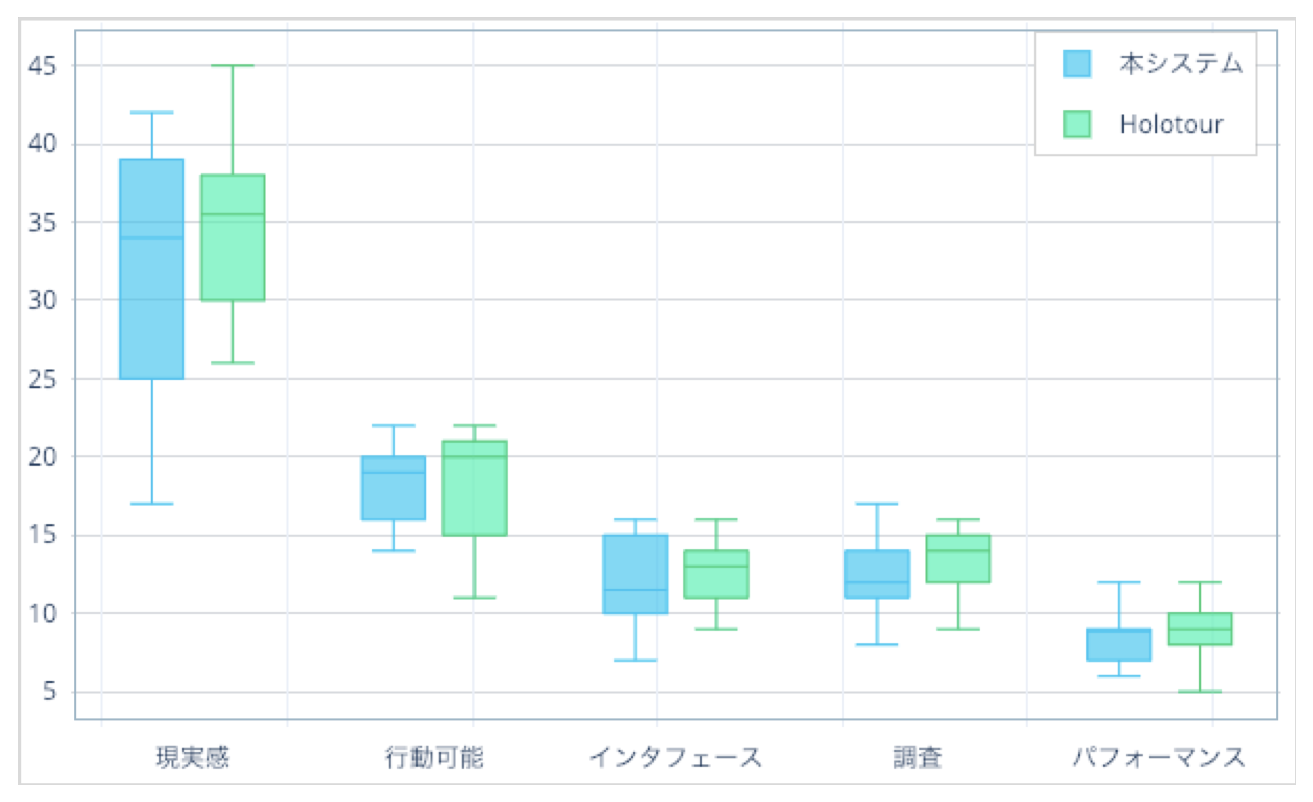
\includegraphics[width=16cm]{img/05_evaluate/result.eps} 
\end{center}
\caption{Presence Questionnaire結果}
\label{figure:pqresult}
\end{figure} 

\subsubsection{現実感}
図\ref{figure:pqresult}ではHoloTourの現実感に関するスコアは最大値,最小値,中央値が本システムよりも高い値となっている.
また2つのシステムの平均スコアを調べたところは本システムが31.8, HoloTourが34.8と平均値がHoloTourの方が高い値となった.
平均値について有意差があるか検定を行った結果, $p$値は0.46であったため本システムとHoloTourの現実感に有意差はみられなかった.

\subsubsection{行動}
%図\ref{figure:pqresult}では
HoloTourの行動に関するスコアは中央値が本システムよりも高い値となっている.しかし,最小値は本システムの方がHoloTourよりも高く,値の差は中央値の差よりも大きい.また最大値は両システムともスコアが22と差はみられなかった.平均を比較すると本システムの平均は18.4, HoloTourは18.0と僅かに本システムの方が高かった.検定を行った結果, $p$値は0.78と有意差はみられなかった.

\subsubsection{インタフェース}
%図\ref{figure:pqresult}では
インタフェースに関してスコアの最大値は本システムとHoloTourで差はみられなかった.しかし,中央値,最小値はHoloTourが本システムよりも高かった.平均を比較すると本システムの平均は12.1, HoloTourは12.7と僅かに本システムの方が低い結果となった.検定を行った結果, $p$値は0.39とこの項目も有意差はみられなかった.

\subsubsection{調査}
%図\ref{figure:pqresult}では
調査に関するスコアの最大値はHoloTourに比べ本システムの方が高かったが,中央値,最小値はHoloTourが本システムよりも高かった.平均を比較すると本システムの平均は12.4, HoloTourは13.6と僅かに本システムの方が低い結果となった.検定を行った結果, $p$値は0.27とこの項目も有意差はみられなかった.

\subsubsection{パフォーマンス}
図\ref{figure:pqresult}ではパフォーマンスに関するスコアの最大値,中央値は同じ値であったが,最小値はHoloTourが本システムよりも高かった.平均を比較すると本システムの平均は8.5, HoloTourは8.9と僅かに本システムの方が低い結果となった.検定を行った結果, $p$値は0.71と有意差はみられなかった.

\subsubsection{ITQとの関係}
図\ref{figure:ITQresult}はPQの各項目の値を縦軸, ITQの値を横軸にとったグラフである.丸い点は本システムのスコアを示しており,菱形の点はHoloTourのスコアを示している.
縦軸方向に青い点と緑の点が離れている時2つのシステムのスコアの差が大きいことがわかる.

\begin{figure*}[t]
\begin{center}
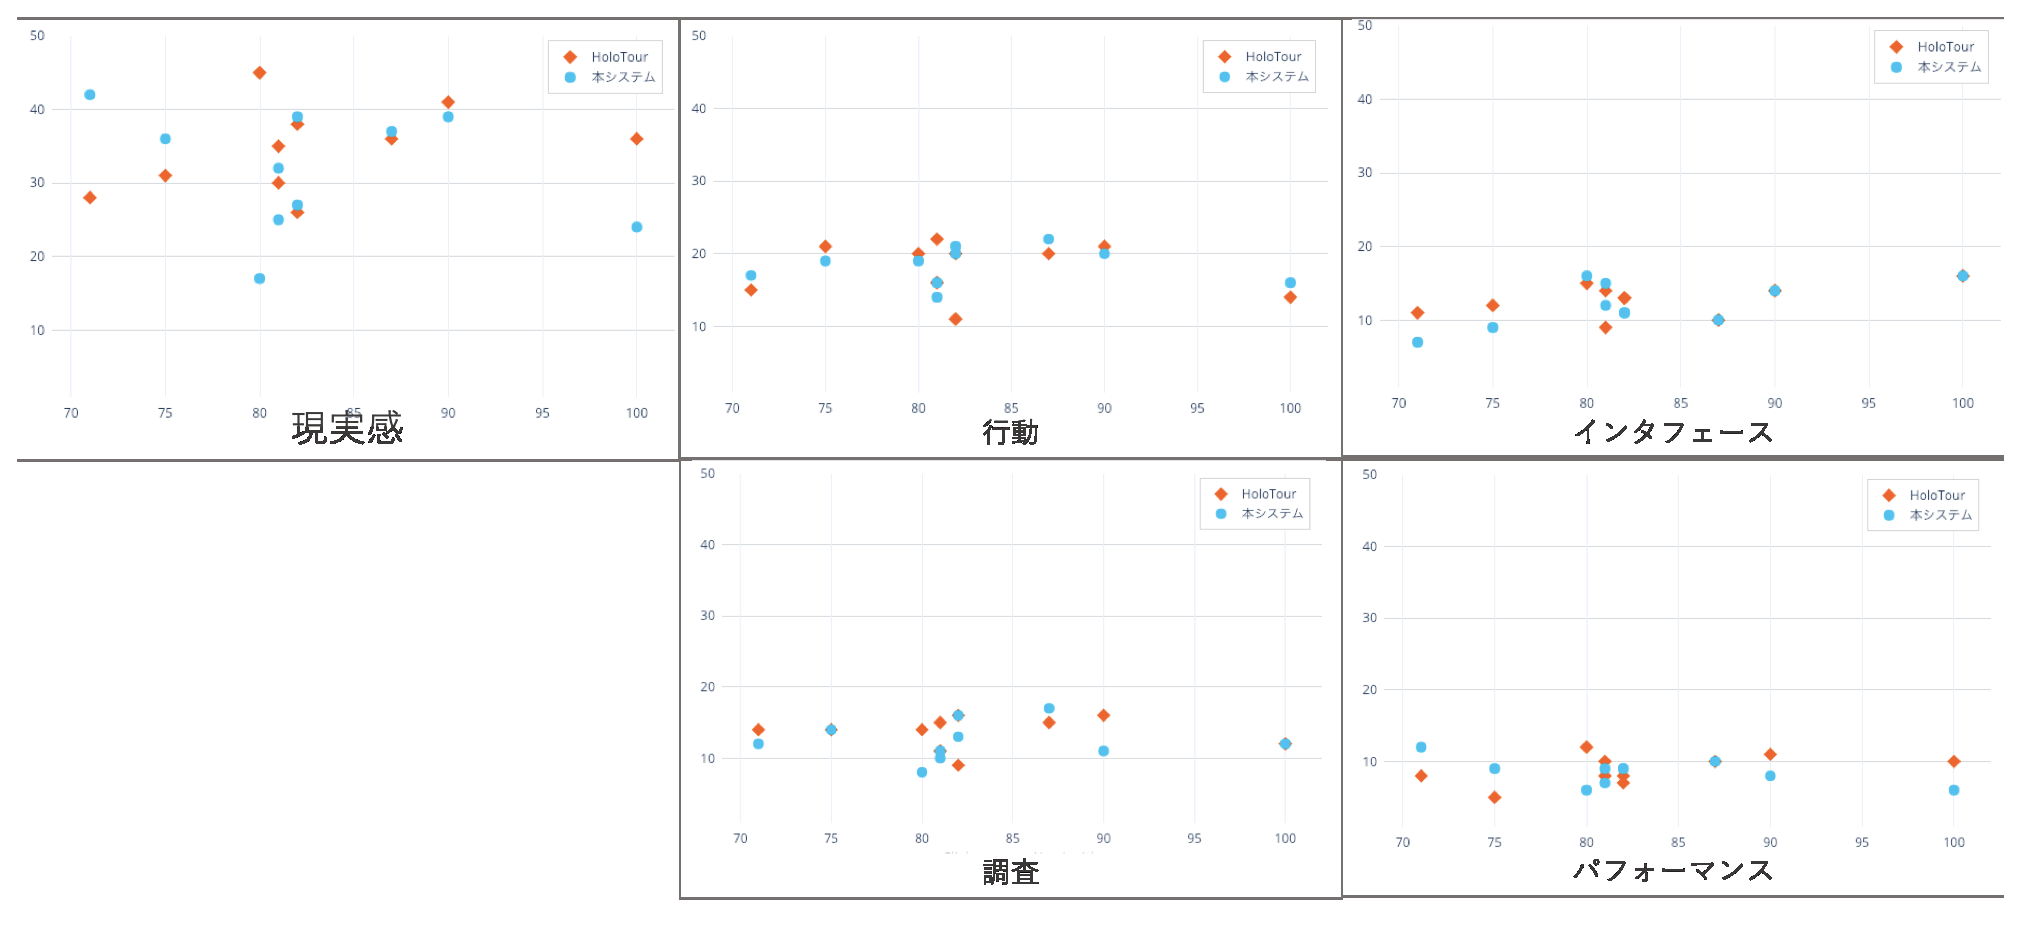
\includegraphics[width=17cm]{img/05_evaluate/ITQresult.eps} 
\end{center}
\caption{PQとITQの関係}
\label{figure:ITQresult}
\end{figure*} 

図\ref{figure:ITQresult}から行動,インタフェース,調査,パフォーマンスのスコアは本システムとHoloTourの間でITQのスコアによる違いはほとんどないことがわかる.しかし現実感に関してITQのスコアが低い被験者ほど本システムを使用した時の方が現実感を高く感じていることがわかる.
逆にITQのスコアが高い人は,本システムよりHoloTourを使用した時により高い現実感を感じている.
本システムよりHoloTourで感じる現実感に高かった被験者はHoloTourのよかったところとして風景が動画で動いているところに現実感を感じていた.逆に本システムの方が現実感があると感じていた被験者に本システムのよかったところを質問したところ,実際に歩くことができることに現実感を感じていた.
\subsubsection{システムについての意見}
被験者に本システムの良いところ,改善してほしいところを質問した.
本システムのよかったところとして遠隔地にいるユーザのアバターに対し親近感を覚えるところや,実際に歩くことができるため没入感が高いとの意見があった.
改善してほしい点として,システムを使用中に音の情報がないことが遠隔地で行動する時の楽しさを減少させているとの意見があった.また風景の更新が遅いことが,実際に遠隔地を歩いている感覚を損ねているとの意見もあった.
\clearpage
\subsubsection{考察}
本システムとHoloTourを比較した時, ITQの値が高い人はHoloTourを使用した際に感じる現実感が高かった.アンケートの回答により表示された風景が動画で出力されていたのが現実感を高める理由であった.そのため没入感を感じやすい人は身体動作よりも視覚情報によって現実感を感じやすいためと考えられる.逆にITQの値が低い人は,視覚情報より身体動作によって現実感を感じるため, HoloTourより本システムを使用した方がより現実感を感じることができたと考えられる.

本システムのよかったところを質問したところ実際に歩くことができる点をあげた人が多かったため,移動を伴う環境でのテレイグジスタンスが現実感を高めるのに有効であると考えられる.
またシステム開発当初は実際の風景と見える 風景が異なるために危険性が懸念されたが,結果的にどの 被験者達からも問題視する声は無かった.これは道路部分を切り抜いた事で現実世界の一部を視認する事ができる事に加えMRによるアプローチが風景表示用球体オブジェクト内の物体も視認できる事が衝突の危険を抑制したためと考えられる.更に本システムで使用したHololensの視野角は35度程度であるため,現実の環境を認識しやすかったことも理由の1つと考えられる.本問題は重要なので今後より精密に評価を行う予定である.

さらにシステムの改善してほしいところを質問したところ,音がなく寂しいところや風景の更新がスムーズに行われないところをあげるユーザが多かった.我々は音をHololensの内蔵スピーカーによるガイドや他ユーザの声の出力,風景更新時のサーバとの通信回数削減によりこれらの問題を解決する.


\clearpage

%7 成果
%7 成果
\section{成果}
%時間の錯覚効果を利用し, 就寝時刻を理想の時刻に近づけることが可能となった.
%しかしながら, 自然に就寝に誘うという目標の達成は不十分であった.
本論文では移動を伴う環境下において遠くにいる人とともに遠隔地の風景での行動を可能にするテレイグジスタンスの手法を提案し,実装したシステムにより評価を行った.
その結果移動など身体動作を伴ったテレイグジスタンス システムは,ITQのスコアが低く没入感を感じにくいユーザに対して有効であることがわかった.
\clearpage

%8 今後の課題
%8 今後の課題
\section{今後の課題}
得られた今後の課題を以下に羅列する.

\begin{description}
	\item[危険性に関する評価]\mbox{}\\
	    評価実験において他者との衝突などの危険性を感じた被験者はいなかった.
	    本研究で実装したシステムはHololensを使用しており,視野角が35度程度と出力範囲が狭いために現実空間の視認がしやすかったためと考えられる.今後の技術革新で視野角が広がり表示範囲が広くなった時,本手法が衝突などの危険性を回避するのに有効かを評価する必要がある.
	\item[音声情報の付与]\mbox{}\\
		学生に対する評価実験において「周囲の環境音がないため寂しい」との意見があった.そこでHololensの内臓スピーカから周囲の環境音を出力する.
	\item[風景更新処理の改善]\mbox{}\\
        現在のシステムは風景の更新処理がスムーズに行われない.そこでサーバとの通信回数の削減によりこの問題を解決する.
%	\item[遠隔旅行コース設定ページの改良]\mbox{}\\
	
\end{description}

\clearpage

%9 謝辞
%9
\section{謝辞}
本研究を行うにあたって多くの方々に協力いただきました.
研究開始から論文執筆まで長期に渡りご指導いただいた濱川礼先生には多大なご協力を頂きました.
また,本論文の副査をお引き受けくださった 本学山田雅之先生,瀧先生に感謝いたします.

本研究室を卒業した村井良行様にはシステム開発中にサーバの通信手法についてアドバイスをいただきました.そのアドバイスのおかげで本システムはより良いものになったと思い, ここに感謝いたします.

更に夏場,冬場共に気温が厳しい中屋外で評価実験に協力していただいた濱川研究室の皆様に感謝いたします.


\clearpage

%10 開発環境
%10
\section{開発環境}
以下に本システムで用いた開発環境を記す.

\subsection{風景表示 アプリケーション}
\begin{table}[htb]
  \begin{tabular}{|c|c|} \hline
    使用デバイス & Hololens \\ \hline
    開発環境 & Windows 10 \\ \hline
    開発ツール & Unity 5.6 \\ \hline
    開発言語 & C\# \\ \hline
  \end{tabular}
\end{table}

\subsection{遠隔旅行コース設定ページ}
\begin{table}[htb]
  \begin{tabular}{|c|c|} \hline
%    使用デバイス & SmartWatch 3 \\ \hline
    開発環境 &  Ubuntu \\ \hline
    開発ツール & Vimエディタ \\ \hline
    開発言語 & JavaScript,Python3 \\ \hline
  \end{tabular}
\end{table}

\clearpage

%11 付録
%11
\section{付録}
付録として本システムの内部仕様設計書, 外部仕様設計書を記載する. 


\clearpage

% 参考文献
\begin{thebibliography}{99}
	\bibitem{telexistence}
S.Tachi, K.Tanie, K.Komoriya, M.Kaneko: Tele-existence (I): Design and Evaluation of a Visual Display with Sensation of Presence; 
Theory and Practice of Robots and Manipulators pp 245-254

\bibitem{factorio}
舘 章:テレロボティクスとテレイグジスタンス; 計測と制御,28巻,12号,p1059-1064

\bibitem{sprots}
Kiana Calagari: Sports VR Content Generation from Regular Camera Feeds; MM'17 Proceedings of the 25th ACM international conference on Multimedia
Pages 699-707

\bibitem{oculus}
Marjolijn Ruyg: Virtual Reality for the Web: Oculus Rift, 2014.

\bibitem{vrmodel}
Randy Hudson: PanoVR SDK―a software development kit for integrating photo-realistic panoramic images and 3-D graphical objects into virtual worlds; VRST ’97 Proceedings of the ACM symposium on Virtual reality soft- ware and technology, Pages 147-154.

\bibitem{ogasawara}
テレイグジスタンス (R) 技術を活用した遠隔操作ロボットの量産型プロトタイプMODEL Hを開発 および、ロボット旅行体験イベントの実施,Telexistence株式会社,KDDI株式会社\\
https://news.kddi.com/kddi/corporate/newsrelease/2018/05/29/3168.html

\bibitem{kinect}
Kinect
https://developer.microsoft.com/ja-jp/windows/kinect,Microsoft.

\bibitem{photon}
Photon Unity Cloud;\\ https://www.photonengine.com/en-US/photon,ユニティ・テクノロジーズ.

\bibitem{gsv}
Google Street View,\\
https://www.google.co.jp/intl/ja/streetview/,Google.

\bibitem{doorcom}
濵上 宏樹, 吉野 孝: ドアコムAR:ポータルを用いた空間接続表現手法
による対話相手の存在感の強化; 情報処理学会インタラクション2018, 

\bibitem{Hololens}
Hololens,\\
https://www.microsoft.com/ja-jp/hololens,Microsoft.

\bibitem{holopotation}
Ben Cutler, Spencer Fowers, Wayne Chang, Samuel Ogden:Holoportation;\\ https://www.microsoft.com/en-us/research/project/holoportation-3/

\bibitem{kiosk}
Devid Debult. SimSensei Kiosk: A Virtual Human In- terviewer for Healthcare Decision Support. Proceedings of the 13th International Conference on Autonomous Agents and Multiagent Systems (AAMAS 2014), May 5-9, 2014.

\bibitem{digitalemily}
Oleg Alexander. The Digital Emily Project: Achieving a Photorealistic Digital Actor. IEEE Computer Graphics and Applications, 2010.

\bibitem{maryam}
Maryam Mustafa. How Human Am I? EEG-based Eval- uation of Animated Virtual Characters. CHI 2017, May 06 - May 11, 2017, Denver, CO, USA, 2017.

\bibitem{shenchang}
Shenchang Eric Chen: QuickTime VR -An Image-Based Approach to Virtual Environment Navigation; SIGGRAPH ’95 Proceedings of the 22nd annual conference on Computer graphics and interactive techniques, Pages 29-38.

\bibitem{fitnamo}
 Edward Nguyan. Fitnamo: Using BodyData to Encourage Exercise through Google Glass CHI 2014, One of a CHInd, Toronto, ON, Canada.

\bibitem{pokego}
ポケモンGO,\\
https://www.pokemongo.jp/ ,https://www.pokemongo.jp/, ナイアンティック,株式会社ポケモン.

\bibitem{mrgame}
Michael Bonfert. 2017. Augmented Invaders: A Mixed Reality Multiplayer Outdoor Game. VRST ’17, November 8-10.

\bibitem{holotour}
David Haley, Danny Askew,Jason Syltebo,Travis Steiner : Case study - Capturing and creating content for HoloTour;\\
https://docs.microsoft.com/en-us/windows/mixed-reality/case-study-capturing-and-creating-content-for-holotour

\bibitem{Unity}
Unity,\\
https://unity3d.com/jp,ユニティ・テクノロジーズ.


\bibitem{json}
JSON,\\
https://www.json.org/json-ja.html

\bibitem{googlemapsapi}
Google Maps API,\\
https://cloud.google.com/maps-platform/?hl=ja,Google.

\bibitem{svrule}
Google Street View 認定要件,\\
https://www.google.co.jp/intl/ja/streetview/earn/, Google.

\bibitem{GSVpano}
GSVPano;\\
https://juampi92.github.io/ GSVPano/.

\bibitem{unitychan}
Unityちゃん,Unity Technologies Japan/UCL\\
https://assetstore.unity.com/packages/3d/characters/unity-chan-model-18705

\bibitem{pq}
Witmer, Singer: The factor structure of the Presence Questionnaire; 298- 312.

\bibitem{itq}
Witmer,Singer: Measuring presence in virtual environments: A presence questionnaire. Presence : Teleoperators and Virtual Environments; 225-240.

%	\bibitem{easing}Andrey Sitnik. ``Easing Function 早見表'' \\ \href{http://easings.net/ja}{http://easings.net/ja}

\end{thebibliography}


\end{document}
